\tikzset{every picture/.style={line width=0.75pt}} %set default line width to 0.75pt        

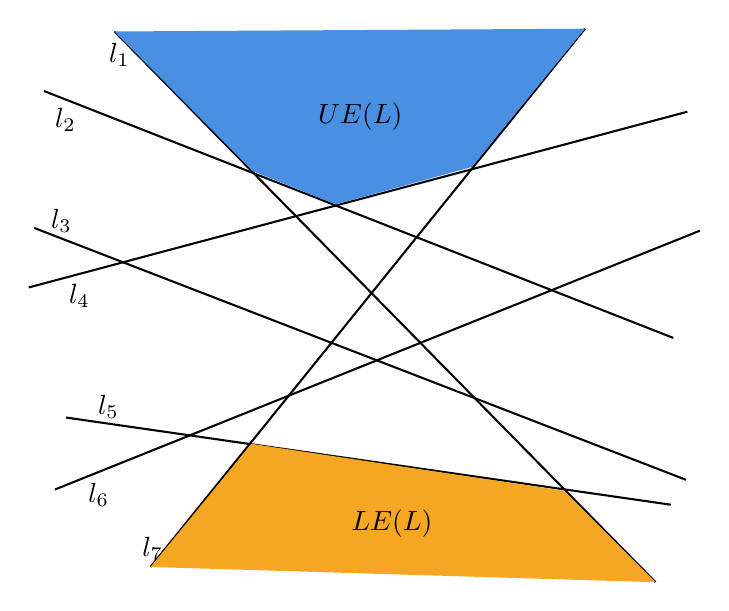
\begin{tikzpicture}[x=0.5pt,y=0.5pt,yscale=-1,xscale=1]
%uncomment if require: \path (0,420); %set diagram left start at 0, and has height of 420

%Straight Lines [id:da8861644180083026] 
\draw    (92.13,398.52) -- (406.13,9.52) ;
%Straight Lines [id:da40732713893670314] 
\draw    (457.13,409.52) -- (66.13,11.52) ;
%Straight Lines [id:da44367949821680464] 
\draw    (468.13,353.52) -- (31.13,290.52) ;
%Straight Lines [id:da2319769205561817] 
\draw    (470,233) -- (15.13,54.52) ;
%Straight Lines [id:da8632177571421473] 
\draw    (480.13,69.52) -- (4.13,196.52) ;
%Straight Lines [id:da43810226035482036] 
\draw    (489.13,155.52) -- (23.13,342.52) ;
%Straight Lines [id:da08264547138329514] 
\draw    (479.13,335.52) -- (8.13,153.52) ;
%Shape: Polygon [id:ds5174786512352558] 
\draw  [draw opacity=0][fill={rgb, 255:red, 74; green, 144; blue, 226 }  ,fill opacity=1 ] (66.13,11.52) -- (406.13,9.52) -- (324.13,109.52) -- (226.13,136.52) -- (166.13,112.52) -- cycle ;
%Shape: Polygon [id:ds7523383015569914] 
\draw  [draw opacity=0][fill={rgb, 255:red, 245; green, 166; blue, 35 }  ,fill opacity=1 ] (391.13,343.52) -- (457.13,409.52) -- (92.13,398.52) -- (165.13,309.52) -- (165.13,309.52) -- cycle ;

% Text Node
\draw (60,17.93) node [anchor=north west][inner sep=0.75pt]  [font=\normalsize] [align=left] {$\displaystyle l_{1}$};
% Text Node
\draw (21,64.93) node [anchor=north west][inner sep=0.75pt]  [font=\normalsize] [align=left] {$\displaystyle l_{2}$};
% Text Node
\draw (18,137.93) node [anchor=north west][inner sep=0.75pt]  [font=\normalsize] [align=left] {$\displaystyle l_{3}$};
% Text Node
\draw (31,191.93) node [anchor=north west][inner sep=0.75pt]  [font=\normalsize] [align=left] {$\displaystyle l_{4}$};
% Text Node
\draw (52,271.93) node [anchor=north west][inner sep=0.75pt]  [font=\normalsize] [align=left] {$\displaystyle l_{5}$};
% Text Node
\draw (45,335.93) node [anchor=north west][inner sep=0.75pt]  [font=\normalsize] [align=left] {$\displaystyle l_{6}$};
% Text Node
\draw (84,374.93) node [anchor=north west][inner sep=0.75pt]  [font=\normalsize] [align=left] {$\displaystyle l_{7}$};
% Text Node
\draw (211,60.93) node [anchor=north west][inner sep=0.75pt]   [align=left] {$\displaystyle UE( L)$};
% Text Node
\draw (235,354.93) node [anchor=north west][inner sep=0.75pt]   [align=left] {$\displaystyle LE( L)$};


\end{tikzpicture}
